\chapter{Introduction to Giraf} \label{ChapIntroduction}
\textit{Giraf is a series of apps for Android, intended to help citizens with autism in their everyday life. Over the past four years Giraf have been under development by students at Aalborg University, with a new group of students taking the mantle every year. As a result of this, it was hard to get an overview of the project in its entirety because we are building upon what others had made. We here give an overview of the Giraf project as it was, when we started working on it, and we also give some insight into the organization of the project.}

\section{Status of Giraf} %To add: pictures to help descripe apps.
At the start of the project all the apps were already released on Google Play, and most of the apps were executable, except for two of the apps which instantly crash upon launch. Most of the executable apps also had some bugs which in could lead to a crash. All of the apps on Google Play were release-versions, but since some of them could not even be executed, it might have been better to have those on the store as alpha or beta-versions.

\section{Multiproject, Subprojects, and Responsibilities} %To add better description of Scrum of Scrums principle.
The overall goal for the multiproject this year was, to make a working system that is usable and stable. A multiproject in this context being an overall project that several groups, in this case all 6th semester software groups, work on in collaboration. In order to achieve a better workflow, the project was split into three subprojects: Database (DB), Graphical User Interface(GUI), and Build and Deployment(B\&D). Our group were a part of B\&D, along with 3 other groups. Both the DB and GUI subprojects had 5 groups each. See Figure \ref{ScrumOfScrumsOverview} for an overview of the structure of the multiproject for this semester.

\begin{figure}
	\centering
	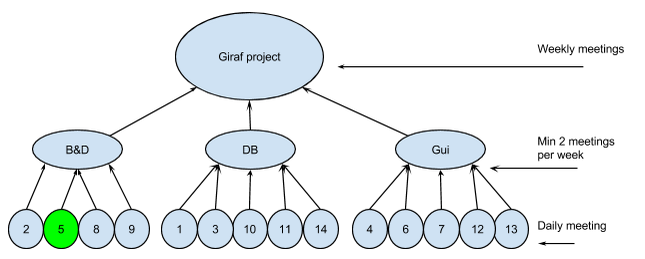
\includegraphics[width=0.8 \textwidth]{pictures/ScrumOfScrum.png}
	\caption{Overview of the initial project structure with subprojects and the individual groups depicted, our group is marked with green.}
	\label{ScrumOfScrumsOverview}
\end{figure}

\subsection{Database}
DB groups were responsible for handling all things database related, this included making current data accessible and adding new data to the database, as per request from other groups or as needed.

\subsection{Graphical User Interface}
GUI groups were mainly responsible for developing the different apps, this included making general changes in the apps and bug fixing anything related to the apps.

\subsection{Build and Deployment}
B\&D groups were responsible for most of the internal project matters, this included maintaining the server services, developing and maintaining the automatic build tools, handling publication of the apps, and administrating the version control. As a B\&D group we had to improve the development environment for the Giraf project.


\section{Project organization}
The project was organized using Scrum principles, where the individual subprojects held Scrum of Scrum meetings twice a week. The individual groups could follow any development method they wanted to, but Scrum was recommended.
In addition, an overall meeting was held every week, where at least one representative from each group were present. At these meetings the overall status for each subproject was given, and any decisions that needed overall consensus were discussed.

As the overall structure was Scrum, the project was split into four sprints. In regards to user stories, it was decided early on at an overall meeting, to operate with two types of user stories, those from the customers, these were called user stories; and those from the other groups, called developer stories. For consistencies sake we will just refer to both as user stories in the report, as the difference was mainly a concern when groups from different subprojects where discussing internally.

\subsection{Group Organization}
Our group used Scrum practices in conjunction with the wider Scrum used in the project. User stories assigned to the group were evaluated using planning poker. Stand-up meetings were held every day. Additionally, we took part in meetings with other groups on subproject and project level. We participated in the project recommendation of being on hand from nine to fifteen every day at the university.

We did not use a burndown chart for our group. Our initial implementation did not pan out for the first sprint, and with our estimations way off and much of our work depending on not being bottlenecked by other groups, we found it to be of too little gain for us. Also, our tasks related to our user stories were not normal. They varied a lot in complexity and time needed to complete them.

\subsection{Roles and responsibilities}
To delegate responsibility of some critical parts of the project, some groups were given roles, so that everyone knew which groups were responsible for what. This way people knew where to go, if there was anything wrong.


\textbf{Process:}
Responsible for ensuring that the overall project follows the scrum principles, and for informing other group about the process used in the project.

\textbf{Configuration Management:}
Responsible for keeping track of the different versions of the apps, and for making sure that only the working version of the apps are released.

\textbf{Google Play:}
Responsible for managing the apps on Google Play, and for making sure they followed the rules set by Google. This was one of our responsibilities.

\textbf{Google Analytics:}
Responsible for managing Google Analytics and ensuring that the crash reports were sent to the groups that requested them. This was also one of our responsibilities.

\textbf{Product Owner:}
This role was given to three groups, one from each subproject. The product owners were responsible for keeping track of the user stories that were assigned to their subprojects, and for organizing the sprint planning sessions and sprint ends. We were product owners for the B\&D subproject.

\textbf{Issue Tracker:}
Responsible for setting up a system on Redmine for keeping track of user stories and for informing group if they do not finish a user story in time or forget to change the status of the user story on Redmine.

\textbf{Server:}
Responsible for the server the project used, this included installing software on the server, upgrading the capacity of the server, and making sure the server was running.

\textbf{Redmine in General:}
Responsible for keeping track of whether the Redmine website was running and for fixing the site if any problems should occur.

\textbf{Redmine Wiki:}
Responsible for keeping the Redmine wiki running and for being the goto group if anyone had problems setting up a wiki page on Redmine.

\textbf{Redmine Forum:}
Responsible for keeping the Redmine forum running.
 
\textbf{Git:}
Responsible for the Git repositories used in the project, and for making changes to it if requested.

\textbf{Webadmin:}
Responsible for keeping the Giraf website running and for updating information on the site when needed. %Insert web link

\textbf{Android Guru:}
This role was given to a person that at the start of the project already had a lot of experience with Android, and worked as a goto guy for anything Android related.

\textbf{Graphics Guidelines:}
This group was responsible for making graphical guidelines for the apps, so that all apps had a consistent look.

\textbf{Code Style:}
This group was responsible for making guidelines for how the code should be written and for writing a guide with common code practices.

\textbf{Customer Representatives:}
This group was responsible for managing the contact between the project and the customers, so that not all groups send them emails all the time and so that if multiple groups have the same question, the question is only asked once.

\section{Tools used in the project}
\textit{In our project we used some tools, to make the whole development process easier and faster. In this section there is a short description of some the the tools used.}

\subsection{Android Studio}
 Android Studio was an IDE made by Google, for coding apps for android devices \citep{AndroidStudio}. We used an older version of Android Studio at the start, but already in the first sprintz into the project Android Studio was upgraded to version 1.0.x.

\subsubsection{Gradle}
To build the project in Android Studio, Gradle was used. Gradle is a project automatic-build tool used by Android Studio, which is designed for use in multiprojects \citep{Gradle}.

\subsubsection{Artifactory}
Artifactory is the maven manager that was used in the project to store and manage versions of the libraries. Because it is able to store multiple versions of every library, it makes it possible to have apps that use an older version of a library and still be able to tell which version is used, and it is also easy to change the version of a library an app is using, by just changing an extension of a line of code in the Gradle build file for the app.

\subsection{Git}
Git was the tool that is used in the project for sharing files internally in the project, primarily code files for the apps. What makes Git good as a file sharing system is that it allows multiple people to code on the same program, and if you commit and another person had committed some changes before you, you can merge the changes between the two versions. Another functionality that Git has that is useful for this project is that it allows the use of “branches”, which allows people to code in a repository that is separate from the original (Master branch).

\subsection{Jenkins}
Jenkins was the tool used for building and testing the apps before release. It was set up so that if anyone pushes changes to the master branch, the app on that branch would be built and then tested by Jenkins. In addition to having tests run every time something is pushed on Git, Jenkins also made an install test and a “monkey test” for all the apps every night. The install test installs all apps on an emulator to test if any of the apps conflicted when installed. The monkey test starts all the apps one by one and then performs random actions to test the stability of the app. When an app is built and tested successfully the new version of the app is pushed to Google Play as an alpha-version.

\subsection{Google Play}
Google Play is the platform on which all the apps are published. By uploading the apps to Google Play the app become available on the Google Play store where everyone that has an android device can find and download them.

\subsection{Google Analytics}
Google Analytics was used in the project to get crash reports from the apps. When an app crashes a crash report is sent to Google Analytics, where you can go and see them. In addition it is also possible to make Google Analytics send the crash report by mail.

\subsection{Redmine}
Redmine is a web-based project management and issue tracking tool \citep{Redmine}, and was used as such in the project. Redmine was in the project used to share user stories and for sharing information in general. This information was shared through a forum and a wiki page. The forum was mostly used to arrange social arrangements and other messages where a little wait time was not a problem, and the wiki page was used for sharing guides, guidelines, general information, and summaries from project meetings.

\subsection{Google Docs}
Like the Redmine wiki, Google Docs was used for sharing information, but only for the project backlog and for summaries from meetings. The reason Google Docs was used for these was that it allowed multiple users to edit the same document simultaneously, so that it was not only one person that was forced to write summaries at the meetings, and for the backlog it allowed one screen to display what was being talked about while another could edit the content.